%!TEX root = ../dokumentation.tex

\chapter{Ergebnis}


\section{Erfolge}

\subsection*{AutomaticDrive}
Die Berechnung und Ausgabe des Lenkwinkels im AutomaticDrive Modus war sehr sinnvoll.
Es lassen sich nun einfach Kamerabilder mit passenden Lenkwinkeln generieren.
Um neue Algorithmen zu testen ist das sehr hilfreich.
Es können auch datenhungrige, Machine Learning Algorithmen bedient werden, da sich die Daten schnell generieren lassen.
Um solche Daten zu generieren ohne Simulation, muss man mit dem Fahrzeug im RC-Modus eine Strecke abfahren, oder man lässt die Fahrzeugsteuerung fahren.
Dies ist deutlich zeitintensiefer.   
\subsection*{Gesamtsimulation}
\begin{center}
    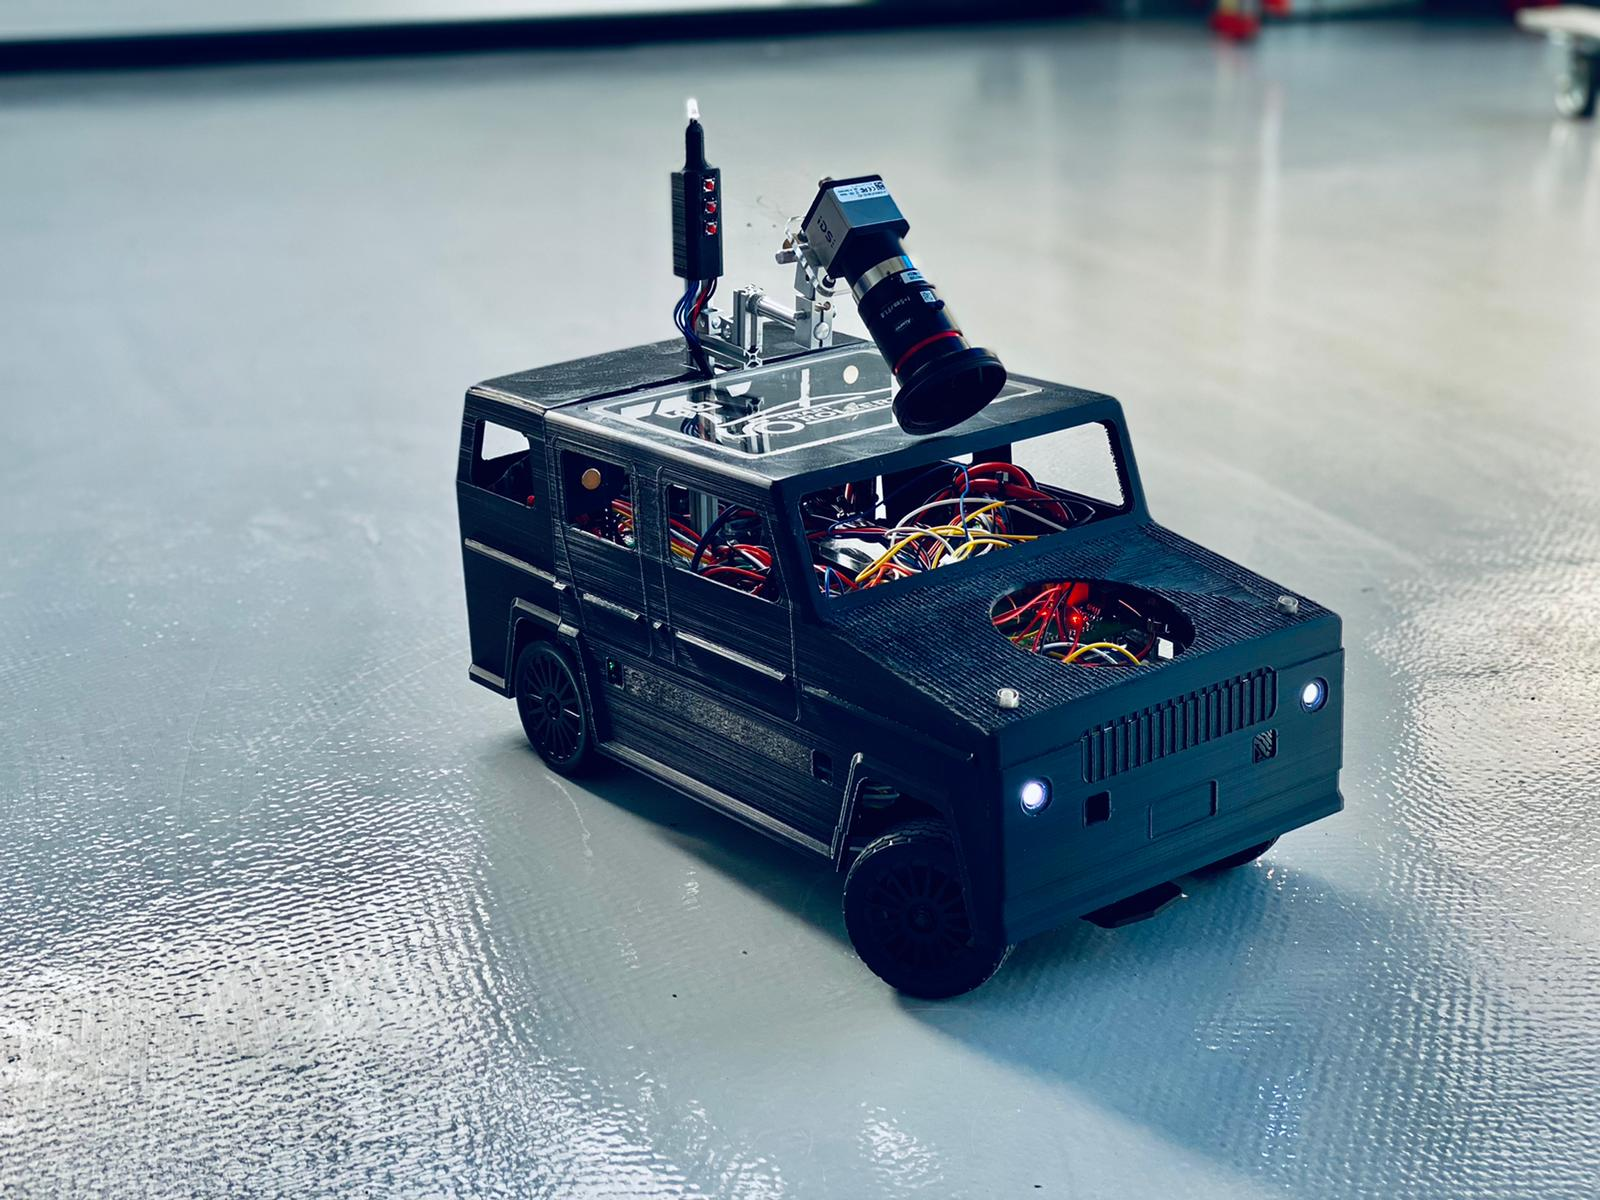
\includegraphics[width=.4\textwidth]{autoFoto.jpg}
    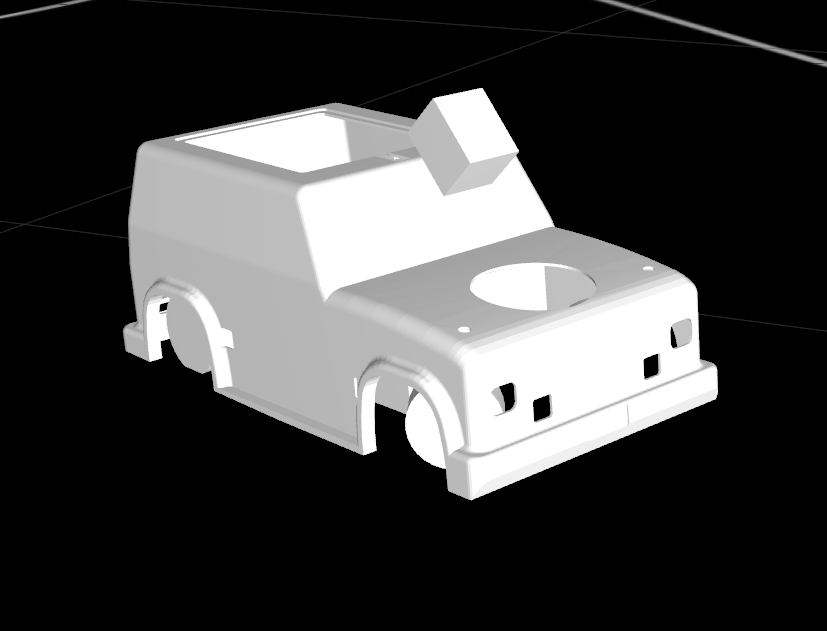
\includegraphics[width=.4\textwidth]{simuFoto.png}
\end{center}
Mit der dynamischen Fahrtsimulation, kann jetzt die Fahrtsteuerung unabhängig von Hardware ausgeführt werden.


\begin{center}
    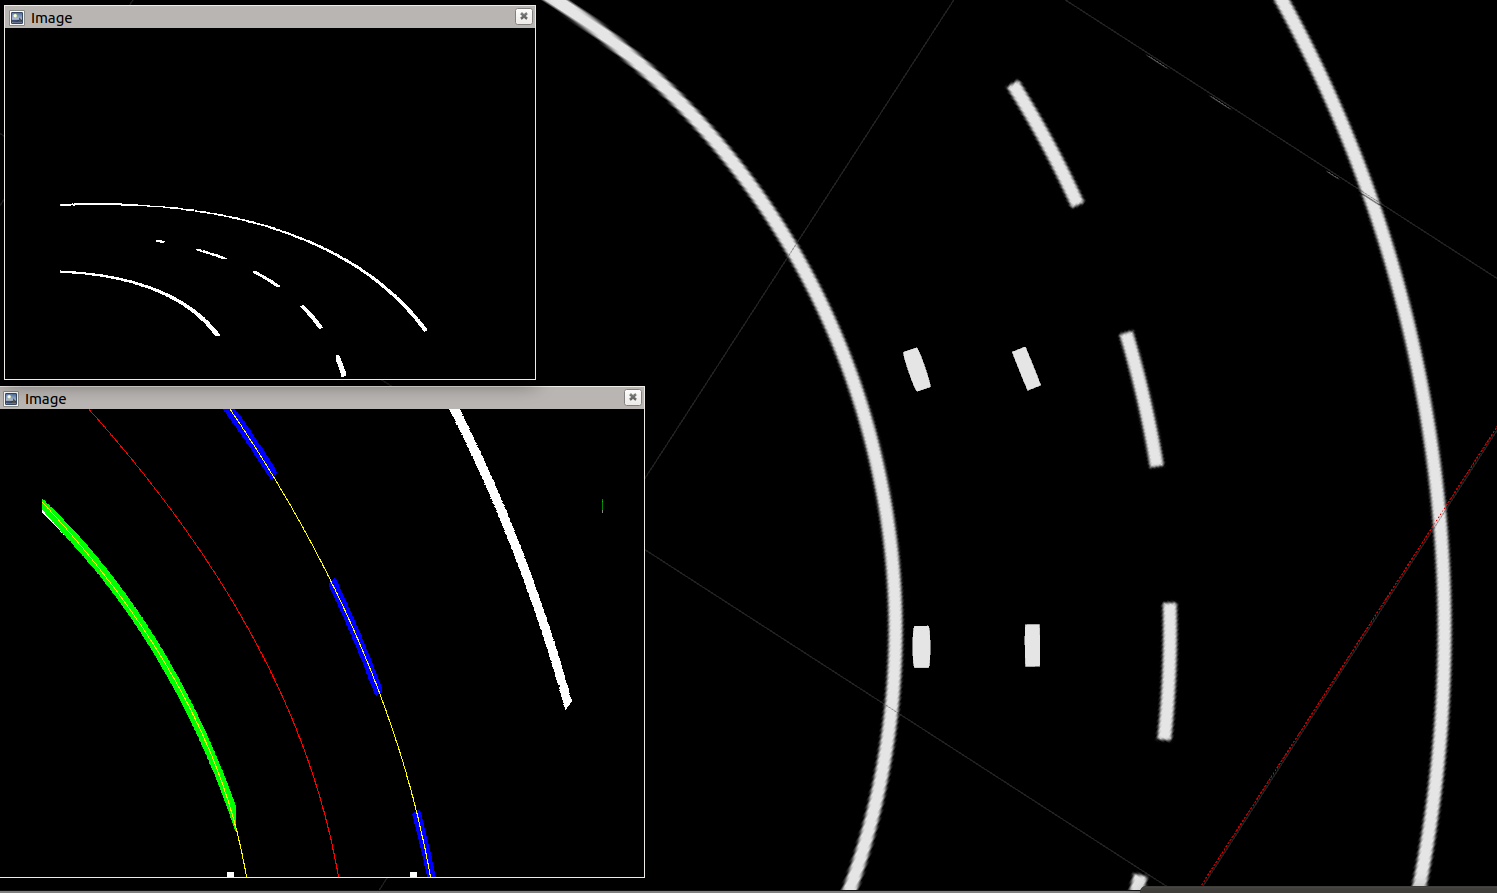
\includegraphics[height=.5\textwidth]{DynamischeLenkung.png}
\end{center}
Dieses Bild zeigt wie die Fahrtsteuerung mit der dynamsichen Fortbewegung funktioniert.
Zur Übersicht sind nur die Räder sichtbar und der Rest des Fahrzeugs ist unsichtbar.
Links oben im Bild sieht man das Kamerabild, welches von der Simulation an die Fahrtsteuerung geschickt wird.
Die Fahrtsteuerung berechnet auf Basis dieses Bildes eine Fahrtrichtung in Form einer Trajektorie.
Unten links sieht man die Trajektorie. Daraus resultiert dann ein Lenkwinkel. 
Der Lenkwinkel wird an die Simulation geschickt. 
Die Simulation passt, bassierend auf dem Lenkwinkel, die Lenkung der Vorderräder an.
Die Räder sind Rechts im Bild zu sehen.


\section{Herausforderungen}
\subsection*{Testen neuer Hardware}
Sensoren wie ToF und Lidar in der Simulation zu testen hat sich nicht gelohnt. 
Die Simulation verhält sich immer noch ein wenig anders als das echte Auto.
Beim Integrieren neuer Hardware hat es sich als besser herausgestellt, Hardwaretests durchzuführen.
Alles was neu in die Simulation kommt, muss in einem langwierigen Prozess immer näher an das Verhalten der echten Hardware angepasst werden.  
\subsection*{Performance}
Wenn sowohl die Fahrzeugsteuerung als auch die Simulation auf meinem Rechner laufen, ist der Rechner ganz ausgelastet.
Wenn es zu wenige Resourcen gibt, berechnet die Fahrzeugsteuerung in größeren Zeitabständen einen Lenkwinkel.
Dadurch kann das Fahrzeug nicht schnell fahren, da es sonst aus der Bahn fährt.
Die Ursache der hohen Performancekosten ist allerdings nicht die Simulation sondern die Fahrzeugsteuerung.
